\documentclass{standalone}

\usepackage{tikz}
\usetikzlibrary{shapes,backgrounds}
\begin{document}

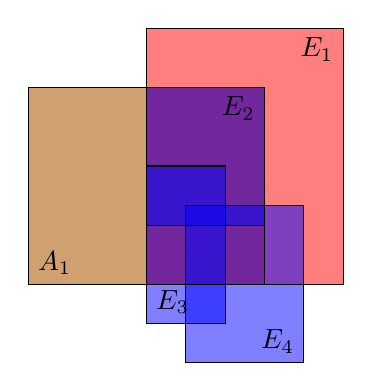
\begin{tikzpicture}

  \def\firstcircle{(0,-0.5cm) rectangle (2.5cm, 2.75cm)}
  \def\secondcircle{(0,0.25cm) rectangle (1.5cm, 2cm)}
  \def\thirdcircle{(1cm, 1cm) rectangle (0,-1cm)}
  \def\fourthcircle{(0.5cm,0.5cm) rectangle (2cm, -1.5cm)}
  \def\taskcircleA{(1.5cm,2cm) rectangle (-1.5cm,-0.5cm)}

  \begin{scope}
      \fill[brown,fill opacity=0.75] \taskcircleA;

      \fill[red,fill opacity=0.5] \firstcircle;
      \fill[blue,fill opacity=0.5] \secondcircle;
      \fill[blue,fill opacity=0.5] \thirdcircle;
      \fill[blue,fill opacity=0.5] \fourthcircle;

      \draw \taskcircleA node[above right] {$A_1$};

      \draw \firstcircle node[below left] {$E_1$};
      \draw \secondcircle node [below left] {$E_2$};
      \draw \thirdcircle node [above right] {$E_3$};
      \draw \fourthcircle node [above left] {$E_4$};

  \end{scope}

\end{tikzpicture}
\end{document}
